%\section{Physics of Dust Devils}
\label{sec:physics}

This chapter addresses what is known about naturally occurring dust
devils, to motivate how best to \textit{engineer} a synthetic version. 
It begins with a qualitative discussion of dust devils, followed by a
review of the known physics and pertinent literature. 
We then introduce a novel concept to leverage these
physical processes as a method of usable, low-grade energy generation.  
The chapter concludes with a brief survey of previous
approaches related to harvesting gravitational potential energy.


\section{Phenomenological Character of Dust Devils}
\label{subsec:phenomena}

There is no rigorous definition of a dust devil, despite the fact that
the phenomenon is ubiquitous. These whirlwinds have been
observed across a wide variety of terrains, climates and even on
other planets\cite{Sinclair1969,Bluestein2004,JGR:JGR13978}. 
While a precise definition is elusive, several features 
are characteristic of a dust devil. These self-sustaining vortices
maintain a funnel-like chimney driven by hot air moving both upward and 
circularly. They are regions of intense rotation, coupled
with upward motions that are strong enough to lift particles into
the flow. It is the entrainment of dust that gives the eponymous
whirlwind its striking visual appearance as a violent coherent
structure.   

While there are characteristic features of a dust devil, they exist over 
a wide range of scales and conditions. They typically survive for
only a few minutes, but they have been observed to endure
hours\cite{ives1947behavior}. The velocities are generally several
meters per second, but 
%
% stolen from: http://glossary.ametsoc.org/wiki/Fujita_scale
%
dust devils are occasionally strong enough to cause damage and injury,
with some reaching F1 on the Fujita Tornado intensity scale, with
velocities between 33 and 49 m/s\cite{fujita1971proposed}. This is
sufficient powerful to result in, ``Surface of roofs peeled off; mobile
homes pushed off foundations or overturned; moving autos pushed off
road``~\cite{Edwards_tornadointensity}.    
%
% dusty! 
% http://clasp-research.engin.umich.edu/e-field/
%
%
% F1 (moderate damage): 33-49 m s-1
%
% ``F1 - Surface of roofs peeled off; mobile homes pushed off foundations
% or overturned; moving autos pushed off road. ``
Diameters range from about one meter to greater than thirty.  Their
average height is on the order of tens of meters, but a few have been
observed as high as one kilometer or more. They do not have a
preferred rotation
direction~\cite{doi:10.1175/1520-0493(1964)092<0363:SPDDM>2.3.CO;2}. Although 
the vertical velocity is predominantly upward, the flow along the a
central axis of large dust devils may be downward. 
%
% cite martian dust devils
%
Visibly similarly structured atmospheric vortices have been observed
over water (Waterspouts), in intense forest fires (Fire Whirls), and in
cold or freezing environments (Snownado). 
%
% good place to ref jacobson2005fundamentals
%
%This is to say nothing of other similar cyclonic phenomena, such as
%tornados and hurricanes. 

While the phenomenon is pervasive, certain environmental conditions
impact the frequency of dust devil formation. 
Sinclair\cite{Sinclair1969} performed perhaps the most 
systematic investigation characterizing conditions favorable for
formation. He noted that dust devils are most
likely to form at solar noon, the time of the greatest incident solar
radiation. Furthermore, they are more likely to form in
locations with a higher surface temperature. Moderate to high wind
speeds (2-5 m/s) encourage dust devil genesis, but greater velocities
(11 m/s) impede formation\cite{JGRE:JGRE1660}. They form more frequently 
in relatively flat locations, such as deserts.   
Despite the name, the lifting of dust does not actually appear to be of
major importance~\cite{Sinclair1969,Sinclair1973,JGRE:JGRE1660}. 
Rather, it is likely that only a small
number of dust devils are visible, and even then, only a fraction of the
actual vortex's physical extent is populated with dust.

%
% more...
%

Actual measurements made inside a dust devil are limited. The available
data hints that dust devils contain two regions: a low surface layer and
a higher inviscid region. These regions are indicated in a 
cartoon in Figure \ref{fig:cartoon}. The low surface region is the
principle location of radial inflow. At the top of this region the flow
reaches its peak velocity, with that peak dropping with increasing
height. The strong radial and azimuthal flow is drawn into a low
pressure core where it gains vertical velocity. Earlier experimental and  
computational studies have observed a ``two-cell'' structure
characterized by a cool downdraft in the center of stronger dust
devils\cite{doi:10.3137/ao.420105,Sinclair1973}. 

The higher region is characterized by a largely inviscid potential flow
with warm air rising and circling around a cool, low pressure
core. This region is typically many times larger in height than the
surface layer. While this region also has radial inflow, it is
significantly weaker than in the lower region. Previous studies have found
this region is relatively well described by a Rankine vortex
model\cite{Sinclair1973,logan1971approach,tratt2003situ}. 

  \begin{figure}[!htb]
    \begin{center}
     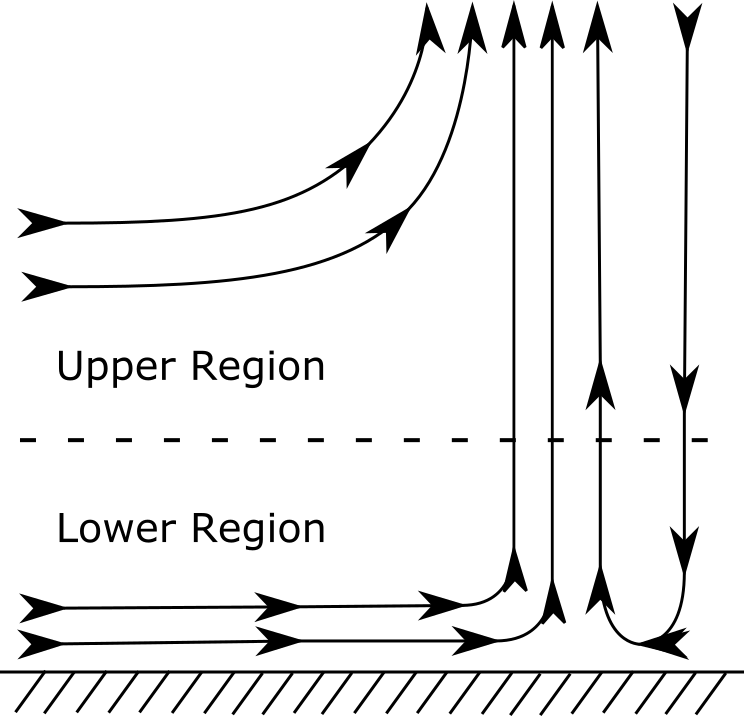
\includegraphics[width = 10 cm]{figs/ground}
     \caption{Cartoon of the structure of a dust devil. The lower region
     is the principle location of radial inflow, with the higher second
     layer flow becoming entrained by the upwardly circulating
     vortex. Notice also the downward flow in the center of the vortex.}
     \label{fig:cartoon}
    \end{center}
  \end{figure}


Renewed interest in naturally occurring dust devils has resulted from
the observation of them on Mars, first photographed by the Viking
Probe~\cite{ryan1983possible}, and more recently by the NASA's Mars
Reconnaissance Orbiter and the Mars rover, Opportunity. Their presence
on Mars, with 1/100 of the atmospheric density of the Earth, speaks to
the universal character of the phenomenon. Due to the greatly decreased
atmospheric density, the Martian dust devils are substantially larger,
ranging several kilometers across at their base and over twenty
kilometers tall\cite{Reiss2016315}. This interest in dust devils and dust
electrification\todo{what does this mean}
 is due to interest in the implications for atmospheric
mixing and transport, and the planned ExoMars Lander will measure
electric fields on Mars\cite{renno_comm}. 

talk about dust devil genesis, cite kanak raleight bernard 
convection and those nice pictures in the genesis les stuff\todo{write me}


The physics of dust devils have also been investigated via numerical simulations.  
While these studies have produced dust
devil like convective vortices, they have been observed in within
existing climate and atmospheric
models\cite{QJ:QJ200513160722,doi:10.3137/ao.420105}, not in simulation 
codes designed specifically to probe the dynamics of a dust devil. 
Many of these results were conducted on numerical grid spacings 
that are typically too coarse
(for instance, 35 meters in the horizontal direction in Kanak's
study\cite{})to generate dust devil's that possess a size consistent
with the observed phenomenon. 

Furthermore, most of these studies are conducted with no mean wind, and
so cannot comment on the impact versus an exclusively thermally driven
vortex\ref{ohno2010mechanisms,kanak2000formation}. 
% mention the grids are not finely resolves
%\cite{smith_leslie,zhao}

It is not clear what generates the azimuthal velocities and there are 
two major hypotheses attempting to explain the behavior. The first is that
that ambient vorticity in the atmosphere is drawn into the vortex from
the far field, and is then intensified due to vortex stretching\cite{?}. %
The other conjecture is that vorticity is generated by
vortex tilting. In this model, the rotation originates by twisting
horizontal vorticity, which is generated by variations in
temperature\cite{?}. %toigo 1-12

%
%Evidence is unclear, for while dust devils are observed to form in
%near-calm conditions, these studies do not discuss the potential
%intensification through this 
%
However, at the time of this writing the origin of
the rotation of a naturally occurring dust devil remains
enigmatic\todo{tilting due to stretching}.  

% RDM:
% note-- tilting due to stretching and horiztonal vorticity
% cannot be a source of vertical angular momentum. 
% you need to evaluate these conjectures, not just report them!
%


%
%kanac has zero wind cases
%

%While dust devils are observed to form in near-calm conditions, these
%studies do not 

\section{Estimate of Dust Devil Power}
\label{sec:estimate_power}

Here we provide a rough estimate of the power
available to a dust devil. There are two objectives of this
analysis. The first is to provide justification for the concept of
extracting power from them, with the reasoning that, should
sufficient power be available, attempting to extract it might be
worthwhile. The second objective is to provide a simple analysis that
can serve as a measure of the efficiency of the generation process,
e.g. ``What fraction of the available power are we extracting?''.  

Steady state conditions requires that the dust devil not
extract more energy than is provided by the thermal resource, the Sun.   
The peak direct solar insolation in Arizona on a hot summer day is
greater than 1000 $W/m^2$. However, this estimate is problematic. 
On one hand it is an optimistic upper bound, as dust devils are only
converting a fraction of this solar resource into kinetic
energy. On the other hand, it is not clear how large of a region
that dust devils draw their energy from. 
Furthermore, Renno and Ingersoll\cite{renno_inger} used an
idealized heat engine frame-work to study natural convection and to
propose a theory for convective available potential energy (CAPE),
and found that the predictions from this substantially underestimate the
observed velocities in the real objects. Finally, dust devils are highly 
intermittent, typically existing only for a short time. It is
not certain that they are accurately represented in a steady
state context. Lending some credence to this are the measurements of
Renno\cite{?} which found that instantaneous surface heat fluxes could
rise to two or three times the average solar insolation. 

Sinclair's anomometer measurements of the velocity profiles inside a dust 
devil provides a more direct estimate. A velocity profile taken 
approximately 9 meters from the ground is shown in Figure
\ref{fig:sinclair_profile}.  

  \begin{figure}[!htb]
    \begin{center}
     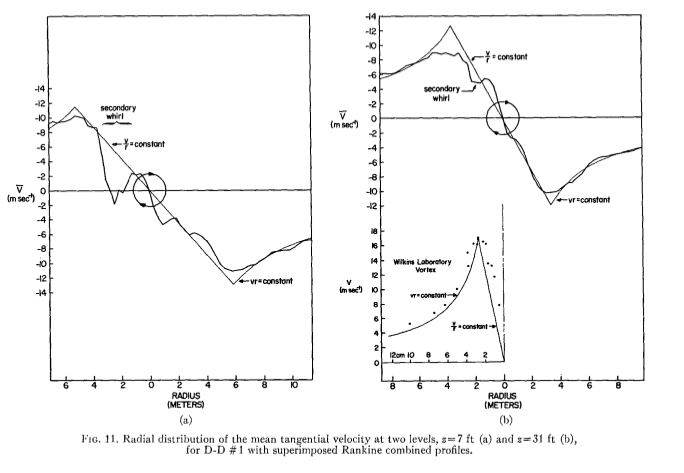
\includegraphics[width = 18 cm]{figs/sinclair_cut}
     \caption{An example of the velocity profiles from Sinclair's 1973
     study of the inner structure of a dust devil. These profiles can be
     integrated to provide a direct estimate of the power contained
     inside one of these objects.}
     \label{fig:sinclair_profile}
    \end{center}
  \end{figure}

This is a dust devil with an inner core radius of approximately 
5 meters, and tangential and axial velocities of 10 m/s, respectively. 
This profile can be integrated to provide an estimate of the kinetic
energy flux though this plane,  
\begin{equation}
 P = -\frac{\rho }{2} \int V_z (V_{\theta}^2 + V_z^2 ) dA, 
\end{equation}
which results in an estimate of 45 kW. This is a substantial amount of
power. This calculation is detailed in Appendix \ref{scaling}. 

%
% show what sinclair measured, then show how we think these energies
% break down into kinetic vs wind
%

As alluded to above, the energy composition of these flows is of
interest. For instance, Carroll and Ryan\cite{JGR:JGR14185} %1970
found that the kinetic energy contained within a dust devil exceeds that
which is attributable to buoyancy. Furthermore, Kaimal and Busigner
observed that dust devils possessed an order of magnitude greater
vertical flux in kinetic energy than similarly sized convective
plumes~\cite{doi:10.1175/1520-0450(1970)009<0612:CSOACP>2.0.CO;2}. The
interplay between rotation, ambient winds and thermal potential energy
are critical to velocity intensities observed in these phenomena. 

As an example of this, consider only the energy flowing into the
entrainment region due to the ambient conditions, in particular, the
incoming wind and heat flowing through a cylindrical control volume
around the dust devil. The dust devil is medium-sized (3m radius) with
an incoming  freestream velocity of 5 m/s. The surface temperature is
343 Kelvin, with a specified inflow boundary layer between the ground
temperature and the ambient air conditions of 313 Kelvin.
%\todo{convert to same as estimate above?}
% cite this?
\footnote{\normalsize These numbers were selected based on information
provided by the Georgia Tech field team from measurements performed in
Arizona during the summer of 2014.} 

In this example, there are two forms of energy to consider: kinetic and
gravitational potential. First, we examine the kinetic energy flux
through the front of the control volume. 
%From the first law of thermodynamics we can express
The kinetic energy flux is a surface integral over the upstream face of
the control volume,  
\begin{equation*}
\text{KE} = \int \frac{\vec V^2}{2} \rho \vec V \cdot \hat n \, dA.
\end{equation*}
%
% could cite fluid dynamics book here
% pg. 239
%
Several simplifying assumptions are made. The freestream 
velocity is assumed to have no components in the span and height and
the variation in height of the streamwise
velocity is only due to the thin boundary layer near the
ground. The boundary layer profile is modeled using the common 7th
power function for a turbulent boundary layer,  
\begin{equation*}
  u(z) = U \text{ min }\left(\left(\frac{z}{\delta}\right)^7,1\right)
\end{equation*}
where U is the constant freestream velocity and $\delta$ the assumed
boundary layer thickness. 
The result for the kinetic energy is then, 
\begin{align*}
\text{KE} & = R \rho U^3 \left[ z_{\text{max}} - \frac{10}{11}\delta
\right].
\end{align*}
Where R is the radius of the vortex. Typical values of these quantities
are, $U = 5$ m/s, $\rho = 1.225$ Kg/$\text{m}^3$, $R = 3$ m,
$z_{\text{max}} = 3$ m and $\delta \approx 10$ cm. This provides an
estimate of 1144 Watts as the incoming kinetic energy flux. 

The gravitational potential energy flux is estimated by integrating the
boussinesq potential energy flux over the upstream flow. 
This is the maximum energy that could be extracted from the flow by an 
adiabatic redistribution of the density variation from the ambient 
density of the freestream flow,
$\rho_\infty$~\cite{hatsopoulos1965principles}. This potential energy  
($E_p$) has the form of a surface integral over the front half of the
control volume, where the ambient winds convect energy across this surface,
\begin{align*}
  E_p & = \int u(z) (\rho(z)-\rho_\infty) g z dA. 
\end{align*}
As the density only varies with height, the integral is simplified to
only vary in this direction,
\begin{align*}
  E_p  & = g \int^{z_\text{max}}_0 u(z) (\rho(z)-\rho_\infty) \, z  \pi
 R \, dz.
\end{align*}
Using the bousinesq approximation, $(\rho(z)-\rho_\infty)  = \rho_0 \beta \Delta T$,
%\begin{align*}
%   (\rho(z)-\rho_\infty) & = - \rho_0 \beta \Delta T 
%   (\rho(z)-\rho_\infty) & = - \rho_0 \beta (T(z) - T_\infty),
%\end{align*}
the integral becomes, 
\begin{align*}
  E_p & = g  \pi R \beta \rho_0 \Delta T \int^{z_\text{max}}_0 u(z) \, z dz.
\end{align*}
This is solved to show
\begin{align*}
  E_p & = g  \pi R \beta \rho_0 U \Delta T \left[ \frac{z_\text{max}^2}{2} - \frac{7 \delta^2}{18} \right].
\end{align*}

%
% \todo{check units}
% 
% lets check the units here--
%
% m/s m^3 1/T kg/m^3 m/s T
%
% = Kg M^2 / s^3
%

%Once again assuming the 7th order power function for a turbulent boundary layer, 
% old text:::
%% \begin{align*}
%%   \text{Potential Energy Flux} & = \int_{-z_\text{max}}^0 u(z) \Delta \rho g z dz. \\
%%   & = \int_{-z_\text{max}}^0 u(z) \rho' g z^2 dz. 
%% \end{align*}
%% Where the substitution, $\Delta \rho = \rho' z$ was made. We again
%% assume the boundary layer follows the 7th order profile, and 
%% that $\rho' = -\beta \rho_0 \Delta T$, resulting in, 
%% %
%% % cite monin-yaglom page 59
%% %
%% \begin{equation}
%%  \text{Power } = U \beta \rho_0 \Delta T g \left[ \frac{z_\text{max}^3}{3} -
%% 					    \frac{7}{30} \delta^3
%% 					   \right]. 
%% \end{equation}

Characteristic values for a dust devil are $\rho_0 = 1.225$ Kg/$\text{m}^3$, 
$\Delta T= 30$ Kelvin, $\beta = 0.003194$ (this is 1/$T_{\text{ground}}$), 
$R = 3 $ m, $z_\text{max} = 2.5$ m, $\delta \approx 10$ cm, $g=9.81$ m/$s^2$, and a
freestream velocity of five meters per second results in an estimate of
103 Watts for the gravitational potential energy flux. 

The majority of the available energy being drawn into the dust devil
region is thus attributable to the kinetic energy of the wind, not the
gravitational potential energy of the air.  
% todo: think about renno
%This is inconsistent with the results of
%Renno\cite{}\todo{missing cite here}, who demonstrated
%that the available thermal energy present was not sufficient to account
%for the velocities measured in dust devils. 
However, while the gravitational potential energy is a small fraction of
the energy available, that does not imply it is without significant
impact. 
%The extent to which the thermal energy acts as an assisting mechanism for 
%``lifting-up'' the flow is unclear, but 
Given the observed increase in dust devil formation during peak thermal
gradients, it is expected to play an important role. The interplay
between the impact on dust devil structure and wind velocities due to
the thermal and wind contributions of energy are examined in detail in
Section~\ref{sec:wind_impact}. 

\section{Dust Devil Generation Concept}
\label{sec:dust_devil_concept}

The discussion in \ref{sec:estimate_power} suggests that dust devils are
carriers of significant kinetic and gravitational
potential energy from the environment. This section provides a brief
discussion on how the physics of naturally occurring dust devils informs
the generation of a synthetic variety, that might be used as a means of
extracting usable work.    

In contrast to the naturally occuring dust devils,
our synthetic solar driven vortex (SoV) design makes use of
control surfaces. These turning vanes also serve as an anchor for the
synthetic vortex, locking it into a small region. An abstract concept of
the turning vane geometry is shown in Figure \ref{fig:cartoon_vanes}.

  \begin{figure}[!htb]
    \begin{center}
     \includegraphics[width = 8 cm]{figs/ground_vanes}
     \caption{Image of a possible two tier turning vane 
       configuration for generating synthetic dust devils. This image depicts a 
       vertical slice through the proposed configuration, and does not show the reflection 
       of the two tier turning vanes, which would be expected to encircle the dust devil core.}
     \label{fig:cartoon_vanes}
    \end{center}
  \end{figure}

% Our observations of the naturally occuring dust devils informs some of
% our \textit{a priori} expectations for the design of the turning
% vanes. The bottom tier are designed to reside in the lower region, where
% the principle inflow will occur. We therefore expect a radial or nearly
% radial start to the vanes, which becomes increasingly tangential as the
% flow moves towards the center. The inner radius of the bottom tier will
% correspond to the outer radius of the generated vortex. 

% The top tier serves a different purpose. We expect a non-zero initial
% angle, as this tier is also designed to protect the rising vortex from
% being blow away by ambient winds. The vanes radius will be shorter, as
% the flow from this tier becomes entrained and the vortex grows in
% size. 

% For both the upper and lower tiers, our objective is to strike a balance
% between effectively turning the incoming flow to impart azimuthal
% velocity, while simultaneously not introducing such a high angle that
% the vanes act as a blocking surface which the incoming flow will move
% around. For instance, when the inlet angles are too severe, the vanes
% block the incoming flow, which results in an adverse pressure gradient
% existing near the outside edge of the 
% vanes. This serves to force fluid around and over the system, instead
% of inside the turning vanes. This reduces the velocity of flow inside
% the system, resulting in a weaker thermal vortex.  To reduce
% the flow blockage, we use gently curving vanes. A gentler angle permits
% more flow to enter the vane region, after which the curvature increases
% toward the center of the vanes. In this way, the angle smoothly varies
% between a nearly zero angle at the outside edge of the vanes to a
% maximum angle at a specified inner radius.

The characteristics of natural dust devils shown in Figure
\ref{fig:cartoon} suggest that the turning vanes be structured with two
tiers (see Figure \ref{fig:cartoon_vanes}). The lower tier would be
designed to manipulate the surface layer 
that lifts up into the core of the vortex, while the upper tier would
control entrainment into the vortex. In both tiers, the design of the
turning vanes must balance between the need to turn the flow from the
radial direction to the azimuthal direction to create vortical motion
and the requirement to not block flow into the vortex. Furthermore, in
the presence of a cross wind, the vanes need to prevent flow that
would pass right through the device and disrupt the vortex.
Finally, in field tests of design concepts for a solar vortex device
conducted by our colleagues at the Georgia Tech, it was found that cross
winds over the facility will also disrupt the vortical flow, and that
this could be controlled by introducing a conical wind-block on top of
the upper tier of vanes. One such field test configuration is shown in
Figure \ref{fig:field_test}. Within this broad conceptual design, there
remains a large design space to explore, including design parameters for
both tiers of vanes and the wind-block cone.

  \begin{figure}[!htb]
    \begin{center}
     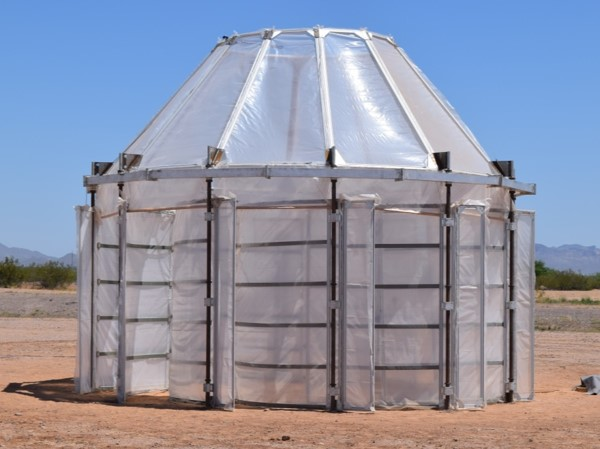
\includegraphics[width = 8 cm]{figs/sov_field}
     \caption{An image of the field configuration from the June, 2015
     tests in Arizona. The second (upper) tier of vanes and the cone are
     clearly visible. This apparatus has an outer diameter of
     approximately six meters.}
     \label{fig:field_test}
    \end{center}
  \end{figure}

To extract energy from the synthetic dust devil formed by the vane
system described briefly above, a turbine would be placed near the top
of the upper vanes. The turbine would extract energy from both the
vertical and azimuthal flow in the vortex, and so the design
considerations are different from those for a classical wind turbine.
Furthermore, there is presumably an analog to the Betz limit on how
much of the energy can be extracted, without disrupting the flow so
much that the vortex cannot be maintained. This is explored as part of
the turbine design process in Section~\ref{subsec:field_predict}. 

In the research conducted here, the design and performance of a dust
devil energy harvesting system are explored using computational
models. Computer models enable a more extensive exploration of
the design space than would be possible experimentally. The design
concepts described above are analyzed to maximize the the
power that can be generated by the system and to develop scaling
describing how power depends on device size, wind speed and thermal
conditions. This has resulted in new design concepts that were also 
evaluated. The subsequent chapter will provide the mathematical
representation used to model the system.  

%
%
%

% Our principle objective is to use a synthetic dust devil to produce 
% usable work. To extract the energy from the synthetic dust
% devil, a turbine is placed 
% at or near the top of the second tier of turning vanes. 
% The blades of the turbine will be driven by the dust devil's azimuthal
% and vertical velocities. While the Betz limit\cite{betz} gives a reasonable
% expectation of the efficiency with which energy can be expected to be
% extracted from the ambient dust devil velocity field, there are other
% non-trivial design considerations. In particular, the impact of the
% turbine on the dust devil's vortex, and any potential disruption of the
% flow on account of the turbine must be investigated. Optimizing the
% turbine to maximize the energy extraction while simultaneously
% minimizing it's impact on the character of the dust devil's solution
% will be an important issue.

% While the turning vanes and turbine  
% paradigm represents a reasonable starting point for design, the
% parameter space of possible system configurations is large. It is
% unclear how to engineer an effective SoV system. Important design
% consideration include: 
% \begin{itemize}
%   \item How should the turning vanes be configured?
%   \item How does the energy produced scale with system diameter?
%   \item Are additional surfaces, such as a cone, capable of increasing energy output?
% \end{itemize}

% Questions such as these provide the principle impetus of using
% computational fluid dynamics (CFD) to inform system design. The
% parameter space of conceivable system designs is far larger than can be
% probed experimentally, and even if such a campaign were to be embarked
% upon, it would be at significantly greater temporal and monetary
% cost. The subsequent chapter will provide the mathematical basis by which
% we model the system, so that we can then begin to discuss how we might
% optimize it computationally.  


\section{Previous Concepts for Extracting Gravitational Potential
 Energy}

%
% essentially an axial flow turbine
%

This is not the first attempt to harness ambient gravitational potential
energy. Rather, a plethora of concepts have been attempted over many
years to generate work from solar energy. 
%Solar chimney. vertical wind mill
%
%
% in fact,
%
Some of the earliest designs for vertical windmills and steam jacks date
back to Roman times\cite{hills1996power}. Leonardo da Vinci sketched a
chimney with a turbine at the top with four
vanes~\cite{lugt1983vortex}. None of these attempts had a lasting impact. 
%for instance steam jack, driven by steam, the smoke jack, driven by hot
%gas rising from the fire are driven by similar principles. 

% 
%Ben Franklin\todo{studied}

%
% solar updraft tower
% https://en.wikipedia.org/wiki/Solar_updraft_tower
%
Modern concepts have been more sophisticated. For instance, solar
updraft towers are envisioned to extract energy from convective hot air
updrafts in the tower by the chimney effect. This airflow drives wind
turbines placed in the chimney updraft or around the chimney base to
produce electricity. A disadvantage of this technology is the
substantial size necessary to produce non-trivial amounts of energy. 
%
% typical solar updraft towers
%
Consider Spain's Manzanares solar chimney, which stands over 200 meters
tall, with a diameter of ten meters. This device collects solar
resource over 250 meters, and has a heat to work conversion efficiency
of 0.2\%\cite{schlaich2005design}. The high cost and complexity of
building structures this tall greatly limit the feasibility of the
concept. These concepts differed greatly from the present work, perhaps
most notably due to the lack of substantial rotation. 

%
% vortex engine
%
A design much closer to the SoV is that of the ``Vortex
Engine''~\cite{vortex_engine,michaud2006atmospheric}. Here, a vortex is
created by admitting warm or humid air tangentially into the base of a
circular wall. This project differs in that the heat source in this case
is waste industrial heat, and the turbine's to extract
the flow occur below the vortex proper, in the radial entrainment
region. Regardless, the core thermodynamic principle is similar.  

Nevertheless, none of these concepts are identical to that investigated
here. In particular, none attempt to harness external winds, nor have
directly turned to the naturally occurring dust devil physics to inform
the design of the apparatus.  
%Finally, in none of these projects has a 

%
% https://en.wikipedia.org/wiki/Vortex_engine
%
%
% https://upload.wikimedia.org/wikipedia/commons/8/8b/Smoke-jack.jpg
%
% http://vortexengine.ca/AVE_FAQ.shtml
%
% http://ir.lib.uwo.ca/etd/89/
%
% http://www.popsci.com/technology/article/2012-12/paypal-cofounder-funds-tornado-harnessing-power-generator-produce-cheap-clean-energy
%
% Philosophies and fallacies in turbulence modeling --citation
%
